\section{Grundzüge der industrierelevanten Verträge}

\subsection{Vertragstypen Übersicht}

\begin{tabular}{l|l|l|l}
Veräusserung & Gebrauchsüberlassung & Arbeitsleistung &
Übrige\\\hline
Kaufvertrag & AirBnB & Werkvertrag & Lizenzverträge \\
& Darlehen & Arbeitsvertrag & \\
& Mietvertrag & Auftrag & \\
\end{tabular}

\subsection{Verträge auf Arbeitsleistung}

\subsubsection{Arbeitsvertrag (Art. 319-362 OR)}

\begin{description}
	\item[Grundsätze] \mbox{}
	\begin{itemize}
		\tightlist
		\item Verrichtung von Arbeit nach Weisungen des Arbeitgebers
		\item Risiko liegt beim Arbeitgeber
	\end{itemize}
	\item[Lohn] Lohnanspruch
	\item[Auflösung] Kündigungsfrist
\end{description}

\subsubsection{Werkvertrag (Art. 363-379 OR)}

\begin{description}
	\item[Grundsätze] \mbox{}
	\begin{itemize}
		\tightlist
		\item Die Pflicht für einen Auftraggeber ein Werk zu erstellen (bspw.
		Software)
		\item Das Entscheidende bei einem Werkvetrag ist das Resultat
		-> Erfolgsverschulden
	\end{itemize}
	\item[Lohn] Vergütungsanspruch
	\item[Auflösung] Jederzeit, solange Werk nicht vollendet
\end{description}

\subsubsection{Auftrag (Art. 394-418v OR)}

\begin{description}
	\item[Grundsätze] \mbox{}
	\begin{itemize}
		\tightlist
		\item Besorgung von Geschäften im Interesse des Auftraggebers
		\item Weisungsrecht des Auftraggebers
		\item Sorgfältige Ausführung, aber kein Erfolg geschuldet
	\end{itemize}
	\item[Lohn] Falls verabredet oder üblich
	\item[Auflösung] Jederzeit, zwingendes Kündigungsrecht
\end{description}

\subsection{Werkvertrag}

\subsubsection{Mängelrechte}
\label{sec:Werkvertrag-Mängelrechte}
\begin{figure}[H]
	\centering
	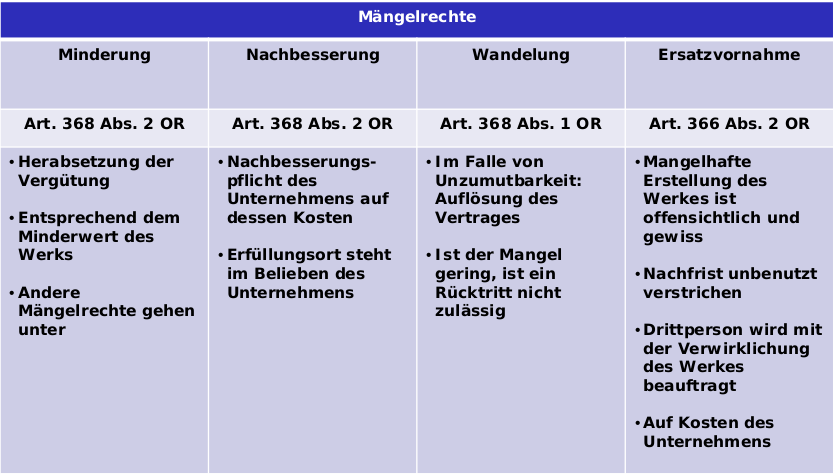
\includegraphics[width=.9\textwidth]{figures/maengelRechte.png}
	\caption{Mängelrechte Werkvertrag}
\end{figure}

\paragraph{Ersatzvornahme}\mbox{}\\
Wird ein Meilenstein während dem laufenden Werkvertrag nicht erreicht,
muss zuerst eine angemessene Nachfrist vereinbart werden. Wird diese
Nachfrist nach wie vor nicht genutzt und verstrichen, kann ein
Dritt-Unternehmen zur Lösung des Problems angestellt werden und die
Kosten müssen durch den Werkvertrag-Nehmer übernommen werden.

\mbox{}\\
Drei Dinge, die bei einem Werkvertrag als erstes beachtet werden
sollten:
\begin{enumerate}
	\tightlist
	\item Zwischen wem ist der Vertrag?
	\item Welches Recht und welcher Gerichtsstand gilt?
	\item Wie komme ich wieder aus dem Vertrag raus?
\end{enumerate}

\subsubsection{Preisvereinbarung}
\label{sec:Werkvertrag-Preisvereinbarung}

\paragraph{Vereinbarter Preis (Art. 373 OR)}
\begin{description}
	\item[Pauschalpreis] Vertraglich fixierter Betrag als Höchst- und
	Mindestpreis.
	\item[Globalpreis] Festpreis (Teuerung angepasst)
	\item[Ausnahme] Missverhältnis zwischen Leistung und Vergütung\\
	Keine Voraussehbarkeit der Umstände.
\end{description}

\paragraph{Fehlende Preisvereinbarung (Art. 374 OR)}

\begin{itemize}
	\tightlist
	\item Wert der Arbeit und der Aufwendungen sind die Vergütungsbemessung
	massgebend (z.B. unverbindlicher Kostenvoranschlag). Ein solcher
	Kostenvoranschlag hat eine gewisse Bedeutung, damit das Kostenrisiko nicht
	ganz auf den Besteller übergeht.
	\item Achtung: Art. 375 Abs. 1 OR: Rücktrittsrecht des Bestellers, wenn
	\textbf{wesentlich} überschritten. (wesentlich = 10\%)
\end{itemize}

\subsubsection{Pflichten des Unternehmners resp. Bestellers}
\label{sec:Werkvertrag-RechtePflichten}

\paragraph{Pflichten des Unternehmers}

\begin{itemize}
	\tightlist
	\item  Pflicht zur Herstellung eines Werks (Art. 363 OR)
	\begin{itemize}
		\tightlist
		\item  Materielles Werk: bewegliche oder unbewegliche Sache
		\item Geistiges Werk: wissenschaftliche oder künstlerische Leistungen
	\end{itemize}
	\item Pflicht zur Lieferung des Werks (Art. 367 OR)
	\begin{itemize}
		\tightlist
		\item Erfolg geschuldet:
		Resultat muss nach obj. Kriterien überprüft und als richtig oder falsch
		qualifiziert werden können
	\end{itemize}
	\item keine besonderen Treuepflichten
\end{itemize}

\paragraph{Pflichten des Bestellers}
\begin{itemize}
	\tightlist
	\item  Pflicht zur Annahme und Abnahme des Werks (Art. 370 OR)
	\begin{itemize}
		\tightlist
		\item  Werkmangel: Vertragliche zugesicherte Eigenschaften fehlen
		\begin{itemize}
			\tightlist
			\item Wertqualität: normale Beschaffenheit
			\item Gebrauchsqualität: normale Benutzung
		\end{itemize}
		\item Prüfungspflicht innert nützlicher	Frist, ansonsten
		Genehmigungsfiktion!
	\end{itemize}
	\item Pflicht zur Leistung einer Vergütung (Art. 363 u. 372 OR)
\end{itemize}

\subsection{Auftrag}
\label{sec:Auftrag-Overview}
Ein Auftrag erfordert eine \textbf{sorgfältige Ausführung}. Es wird jedoch
\textbf{kein Erfolg geschuldet}.

Der Auftrag muss persönlich ausgeführt werden. Andernfalls musst der
Beauftragte den Auftraggeber informieren, falls die ausführende Person
wechselt.

\begin{figure}[H]
	\centering
	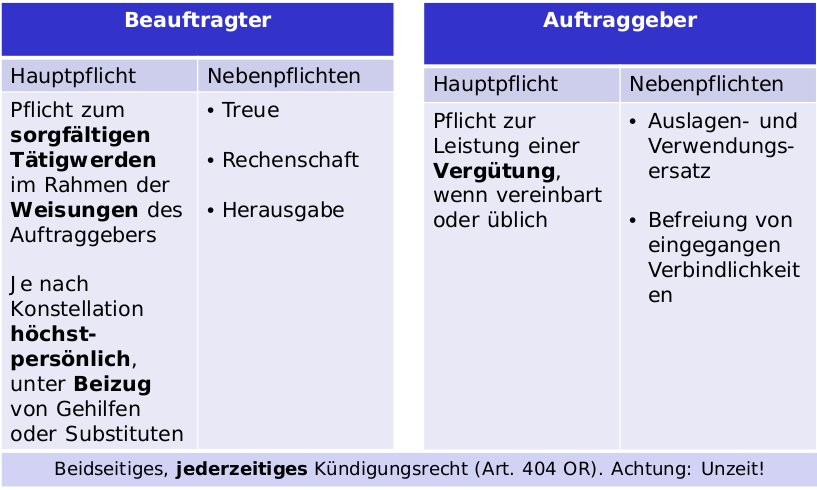
\includegraphics[width=.9\textwidth]{figures/auftraggeberBeauftragter.png}
	\caption{Beauftragter und Auftraggeber}
\end{figure}

\begin{description}
	\item[Herausgabe] Der Arzt z.B. die Dossiers an
	einen neuen Arzt weitergibt oder Informationen zur Verfügung stellt.
	\item[Unzeit] Die Gegenseite kann nicht mehr disponieren.
	\item[Kündigung] Jederzeit, \textbf{unabhängig davon ob Kündigungsfristen
	im Auftrag stehen} oder nicht.
\end{description}


\subsection{Vertragsabschluss}

\subsubsection{Voraussetzungen}

\begin{enumerate}
	\tightlist
	\item \textbf{Rechts- und Handlungsfähigkeit} der Vertragsparteien
	\item Vorliegen \textbf{beidseitigen Geschäftswillen}
	\item \textbf{Austausch übereinstimmender Willenserklärungen}
	\begin{itemize}
		\tightlist
		\item Antrag:
		\begin{itemize}
			\tightlist
			\item Zeitlich erste Willenserklärung bei Vertragsverhandlung
			\item Muss alle für den Vertrag massgebenden Punkte enthalten
		\end{itemize}
		\item Annahme:
		\begin{itemize}
			\tightlist
			\item Zeitlich zweite Willenserklärung bei der Vertragsverhandlung
			\item Antragsempfänger erklärt Willen zum Vertragsabschluss durch die
			Annahme
			\item Inhaltliche Übereinstimmung von Antrag und Annahme notwendig
		\end{itemize}
	\end{itemize}
	\item Einhaltung von Formvorschriften, sofern erforderlich\\
	Gewisse Verträge müssen z.b. schriftlich, öffentlich oder beurkundet
	werden.
	\item Keine Verletzung inhaltlicher Schranken / keine Willensmängel (Art.
	19/20ff. OR)
\end{enumerate}


\subsubsection{Formvorschriften}

\begin{figure}[H]
\centering
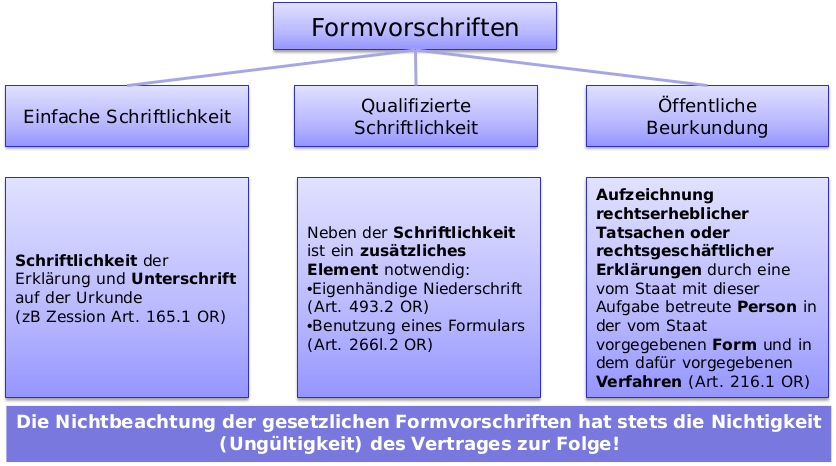
\includegraphics[width=.9\textwidth]{figures/formvorschriftenVertragsabschluss.png}
\caption{Formvorschriften Vertragsabschluss}
\end{figure}

Ein Mail entspricht nicht \textbf{einfacher Schriftlichkeit}.\\
Ein Testament muss z.B. handschriftlich (Qualifizierte Schriftlichkeit)
sein, sonst ist es formnichtig.\\
Eine Kündigung eines Mietverhältnisses durch den Vermieter muss mit
einem offiziellen Formular gemacht werden (Qualifizierte
Schriftlichkeit).

\subsubsection{Vertragserfüllung}

\begin{itemize}
\tightlist
\item Bei der Vertragserfüllung werden die durch den Vertragsabschluss
begründeten Obligationen (Verpflichtungen) erfüllt.
\item Das Internet ist ein neues Kommunikationsmedium, das heute vermehrt
dazu benutzt, übereinstimmende Willensäusserungen auszutauschen, die
zu Vertragsabschlüssen führen (Art. 1 OR).
\item Fragen des Vertragsabschlusses und der Vertragserfüllung regeln sich
-- genau wie beim mündlichen Vertragsabschluss oder beim brieflichen
Austausch von Willenserklärungen -- nach den allgemeinen Bestimmungen
des Obligationenrechts.
\end{itemize}

\subsubsection{Vertragsverletzungen}

\begin{figure}[H]
\centering
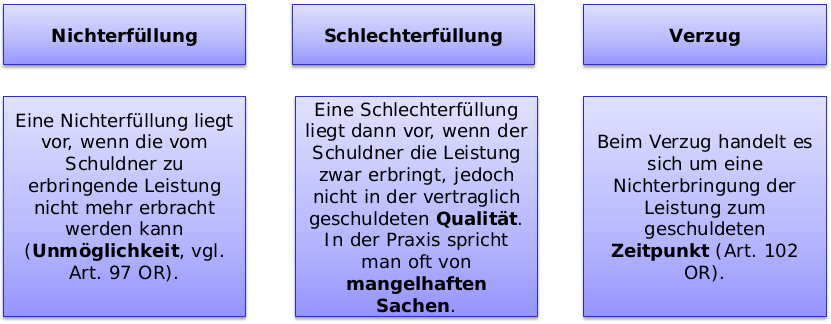
\includegraphics[width=.8\textwidth]{figures/agbVertragsverletzungen.png}
\caption{AGB Vertragsverletzung}
\end{figure}

\textbf{Knonentionalstrafe:} Ist unabhängig ob wirklich ein Schaden
entstanden ist oder nicht. Zudem kann zusätzlich die Vertragserfüllung
trotzdem verlangt werden.

\subsection{AGB}

AGB sind \textbf{vorformulierte} Vertragsbestimmungen, die als Grundlage
für eine Vielzahl von Verträgen verwendet werden, die der Verfasser mit
seinen Kunden schliesst.

Ziele von AGB:
\begin{itemize}
	\tightlist
	\item \textbf{Rationalisierungszweck}
	\item Besserstellungszweck:
	\begin{itemize}
		\tightlist
		\item Freizeichnungs-Klauseln
		\item  Sicherheiten-Klauseln
		\item Risikoverlagerungen
	\end{itemize}
	\item Verhandlungsvorgabe
\end{itemize}


\subsubsection{Einbezug}
Für das Zustandekommen eines Vertrages (Konsens) bedarf es der
übereinstimmenden gegenseitigen Willenserklärungen beider Parteien. Dies
gilt auch für die Einbeziehung der AGB in den Individualvertrag

\paragraph{Voraussetzungen der AGB-Einbeziehung}
\begin{itemize}
	\item AGB-Kundbarmachung:
	Kunde \textbf{ist vor oder während} der Vertragsverhandlungen auf die
	AGB hinzuweisen
	\item AGB-\textbf{Kenntnisnahme}: Kunde muss spätestens vor
	Vertragsschluss Gelegenheit zur Kenntnisnahme haben.\\
	Achtung: Nachgeschobene AGB sind ungültig
	\item AGB-Geltung: Kunde muss mit der AGB-Geltung einverstanden sein.
\end{itemize}


\subsubsection{Typologisierung}
\begin{figure}[H]
\centering
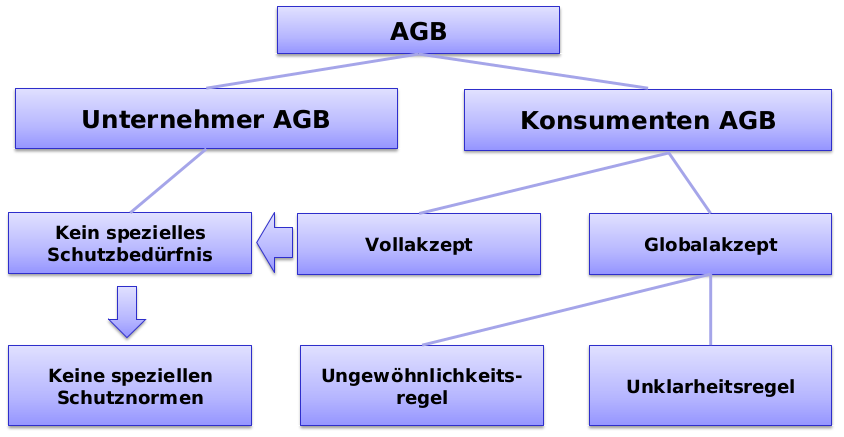
\includegraphics[width=.9\textwidth]{figures/typolisierungAGB.png}
\caption{Typologisierung der AGB}
\end{figure}

\begin{description}
	\item[Globalakzept] Bedeutet, dass viele leute einfach ohne zu lesen
	die AGB akzeptieren. Dann gibt es die beiden folgenden Regeln zu
	beachten.
	\item[Ungewöhnlichkeits- und Unklarheitsregel]
	Verwendung missbräuchlicher Geschäftsbedingungen (Art. 8 UWG) „Unlauter
	handelt insbesondere, wer allgemeine Geschäftsbedingungen verwendet, die
	in \textbf{Treu und Glauben} verletzender Weise zum Nachteil der
	Konsumentinnen und \textbf{Konsumenten} ein erhebliches und
	ungerechtfertigtes \textbf{Missverhältnis} zwischen den vertraglichen
	\textbf{Rechten und Pflichten} vorsehen.``
	\item[Ungewöhnlichkeitsregel]  Enthalten AGB Bestimmungen, mit denen
	der Kunde (nach Treu und Glauben) nicht rechnen muss, so sind diese
	Bestimmungen für den Kunden nicht verbindlich\\
	\emph{z.B. in einem Ski-Hüttchen der Gerichtsstand in Florida}
	\item[Unklarheitsregel] Finden sich in den AGB Regelungen, die unklar
	sind, so werden diese zu Lasten des Verfassers der AGB ausgelegt.\\
	\emph{Wenn der Leser etwas der AGBs nicht versteht (oder verstehen
	kann), werden diese Teile zu Lasten des Verfassers ausgelegt.}
\end{description}


\subsection{SIA-Verträge}

\begin{itemize}
	\tightlist
	\item Vertragsformulare der SIA für Geschäftsbeziehungen zwischen
	\begin{itemize}
		\tightlist
		\item \textbf{Bauherren und Planern} (Aufträge) sowie zwischen
		\begin{itemize}
			\tightlist
			\item BSP: Vertrag für Ingenieurleistungen Nr. 1003
		\end{itemize}
		\item \textbf{Bauherren und Unternehmern} (Werkverträge)
		\begin{itemize}
			\tightlist
			\item BSP: Werkvertrag Nr. 1023
		\end{itemize}
	\end{itemize}
	\item Sicherstellung der \textbf{korrekten Einbindung} der entsprechenden
	Vertragsnorm
	\item \textbf{Breit abgestützte Grundlage} für die Geschäftsbeziehung
	\item Schweizweit anerkannt und für \textbf{80\% der Fälle als Standard
	anwendbar}
	\item Knappe und \textbf{klare Struktur} / detaillierte Aspekte mithilfe von
	Beilagen
\end{itemize}

\subsection{SWICO-Verträge}

\begin{itemize}
	\tightlist
	\item IT-Modellverträge, welche durch Anwälte der Verbände SWICO und
	SwissICT erarbeitet werden
	\item Faire und ausgewogene Regelungen
	\item Konkrete Bezugnahme auf IT-relevante Vertragsgestaltungen
	\item Nur Geltung, wenn konkret im Vertrag vereinbart
\end{itemize}

\textbf{Vorteile Swico-Verträge}

\begin{enumerate}
	\tightlist
	\item Branchenbezogenheit
	\item Fachgerechte Formulierung
\end{enumerate}
